\subsubsection{Análisis para $C_{comp_{4}}$ en modo corriente, $I_{out} = 200 \si[per-mode=symbol]{\milli\ampere}$, $R_{L} = 0 \si[per-mode=symbol]{\ohm}$}

Se puede ver en la figura~\figref{fig:fig_power_supply_CCOMP4_LOOP_Modo4} como ya con el valor de $C_{comp_{4}} = 10 \si[per-mode=symbol]{\nano\farad}$ se logra unos márgenes de fase y ganancia aceptables, valores menores directemente dan negativos, además seguir aumentando el valor de $C_{comp_{4}}$, no cambian mucho el ancho de banda de la respuesta en frecuencia, pero presenta sobre-pico de resonancia y  la fase empeora, como se puede ver en la figura~\figref{fig:fig_power_supply_CCOMP4_RF_Modo4}. A nivel de respuesta dinámica el comportamiento es inverso respecto al tiempo de crecimiento, ver figura~\figref{fig:fig_power_supply_CCOMP4_STEP_1n_Modo4}, figura~\figref{fig:fig_power_supply_CCOMP4_STEP_10n_Modo4} y figura~\figref{fig:fig_power_supply_CCOMP4_STEP_100n_Modo4}.

\vfill


% CCOMP4 MODO 4.

\clearpage

\begin{figure}[H] %htb
\begin{center}
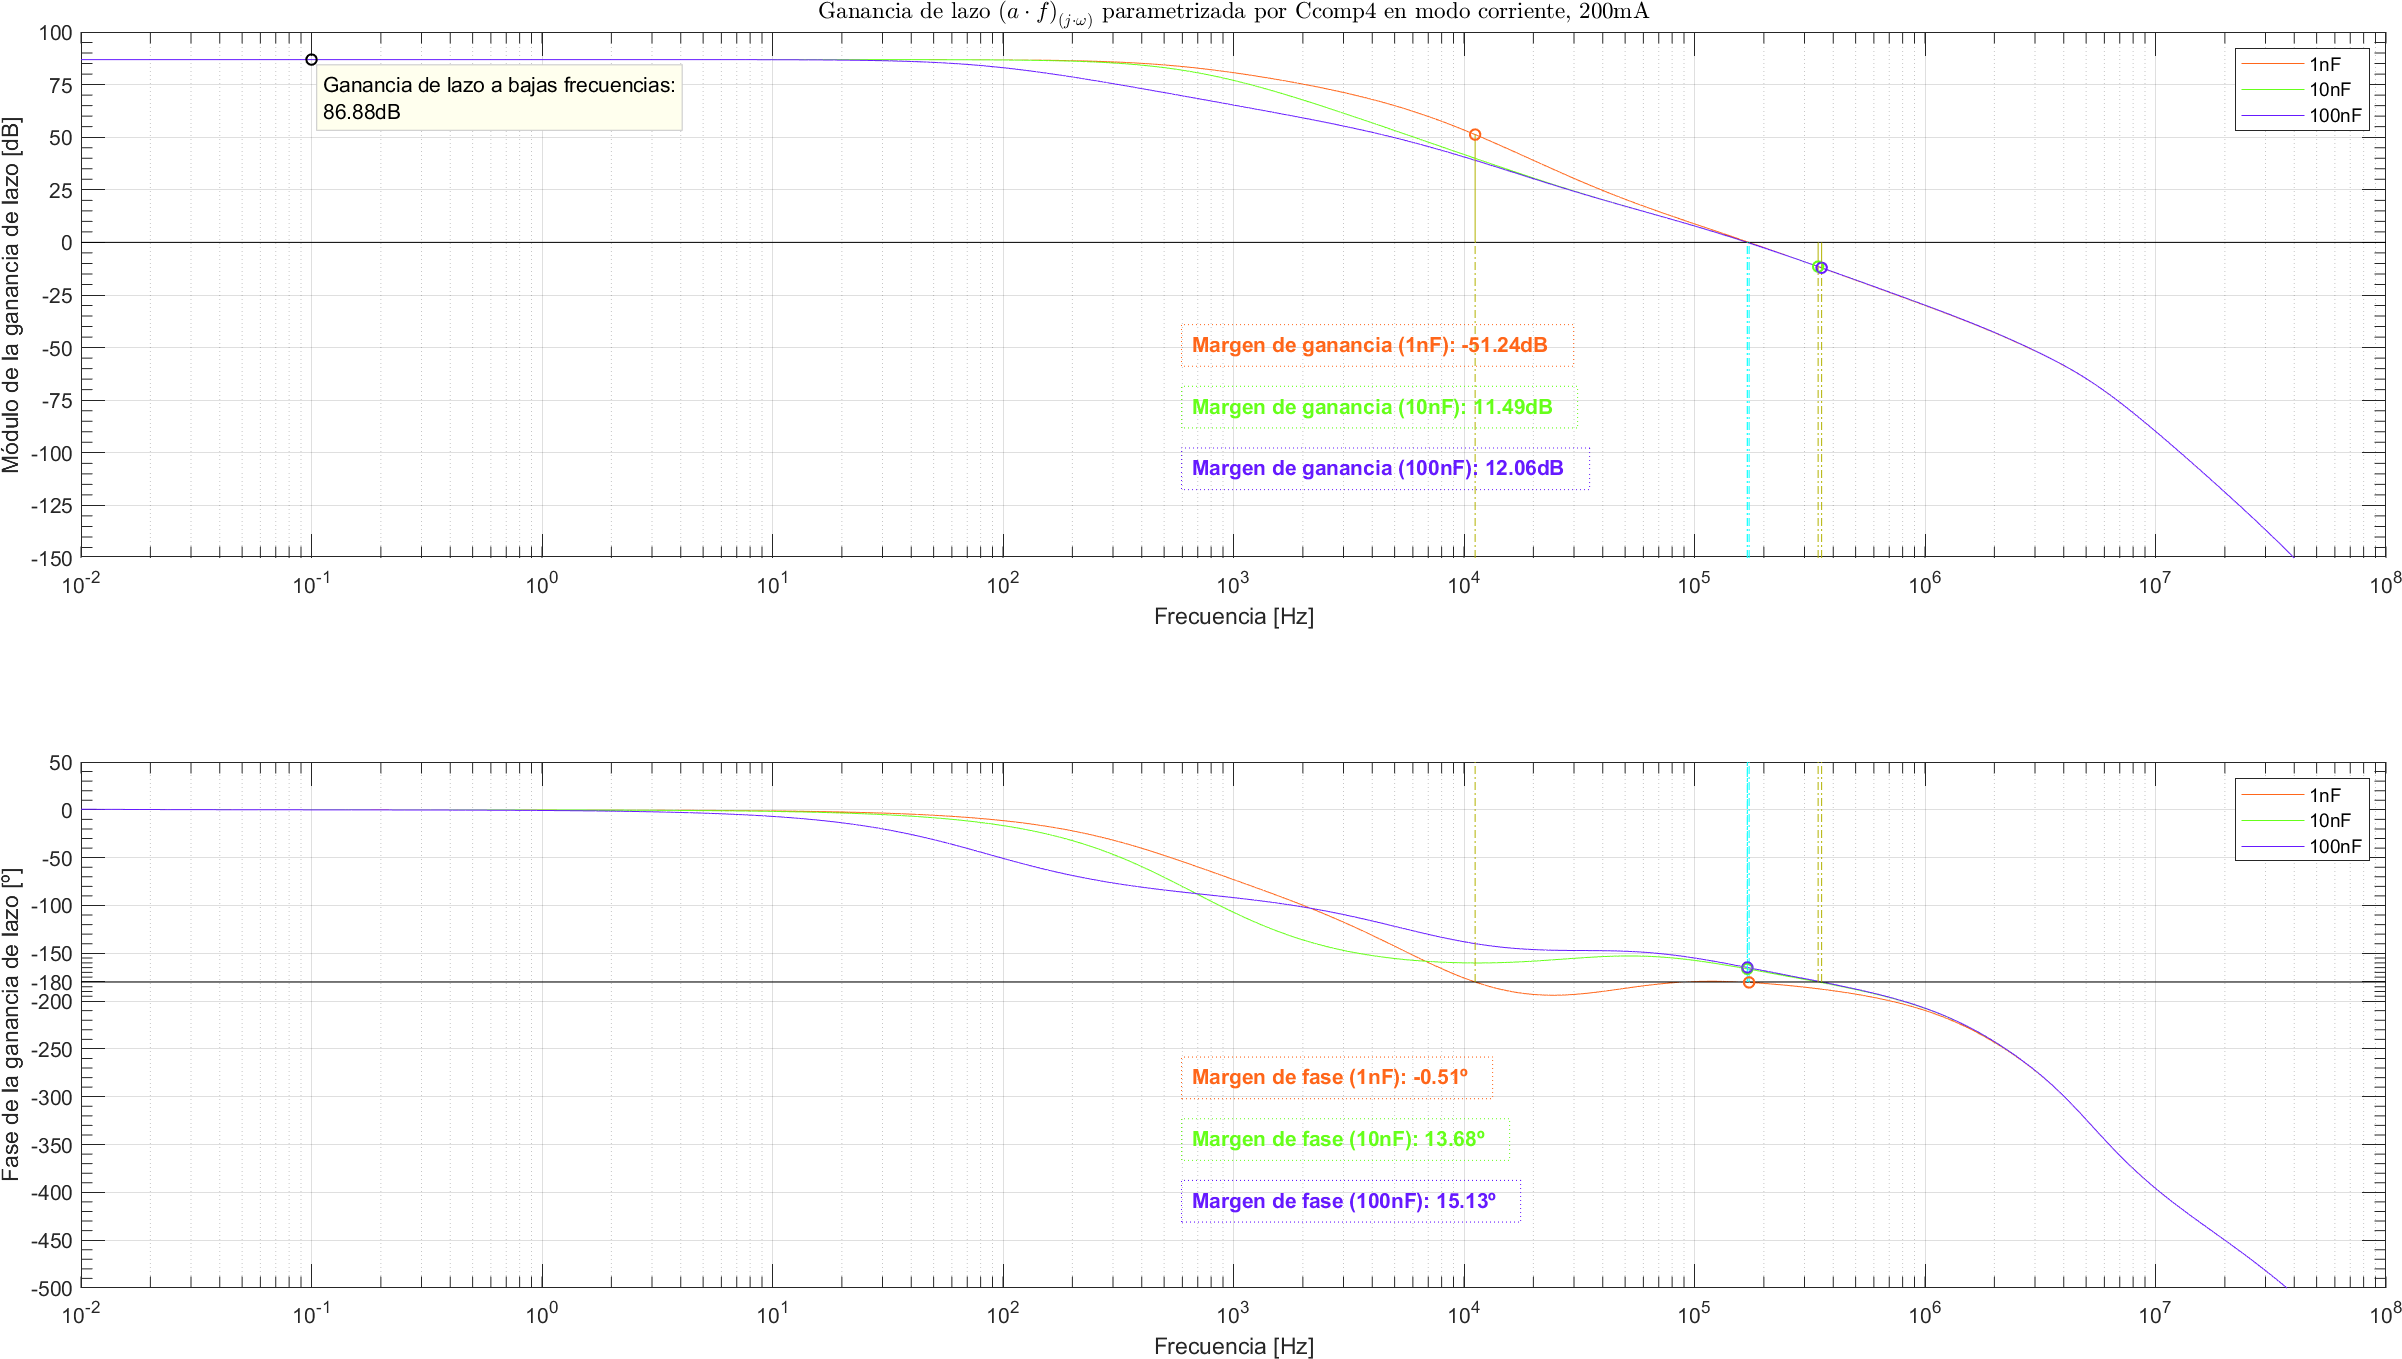
\includegraphics[width=1.1 \textwidth, angle=90]{./img/plots/loop/power_supply_CCOMP4_LOOP_Modo4.png}
\caption{\label{fig:fig_power_supply_CCOMP4_LOOP_Modo4}\footnotesize{Ganancia de lazo en modo corriente, $I_{out} = 200 \si[per-mode=symbol]{\milli\ampere}$, en función de la frecuencia parametrizada por $C_{comp_{4}}$.}}
\end{center}
\end{figure}


\clearpage

\begin{figure}[H] %htb
\begin{center}
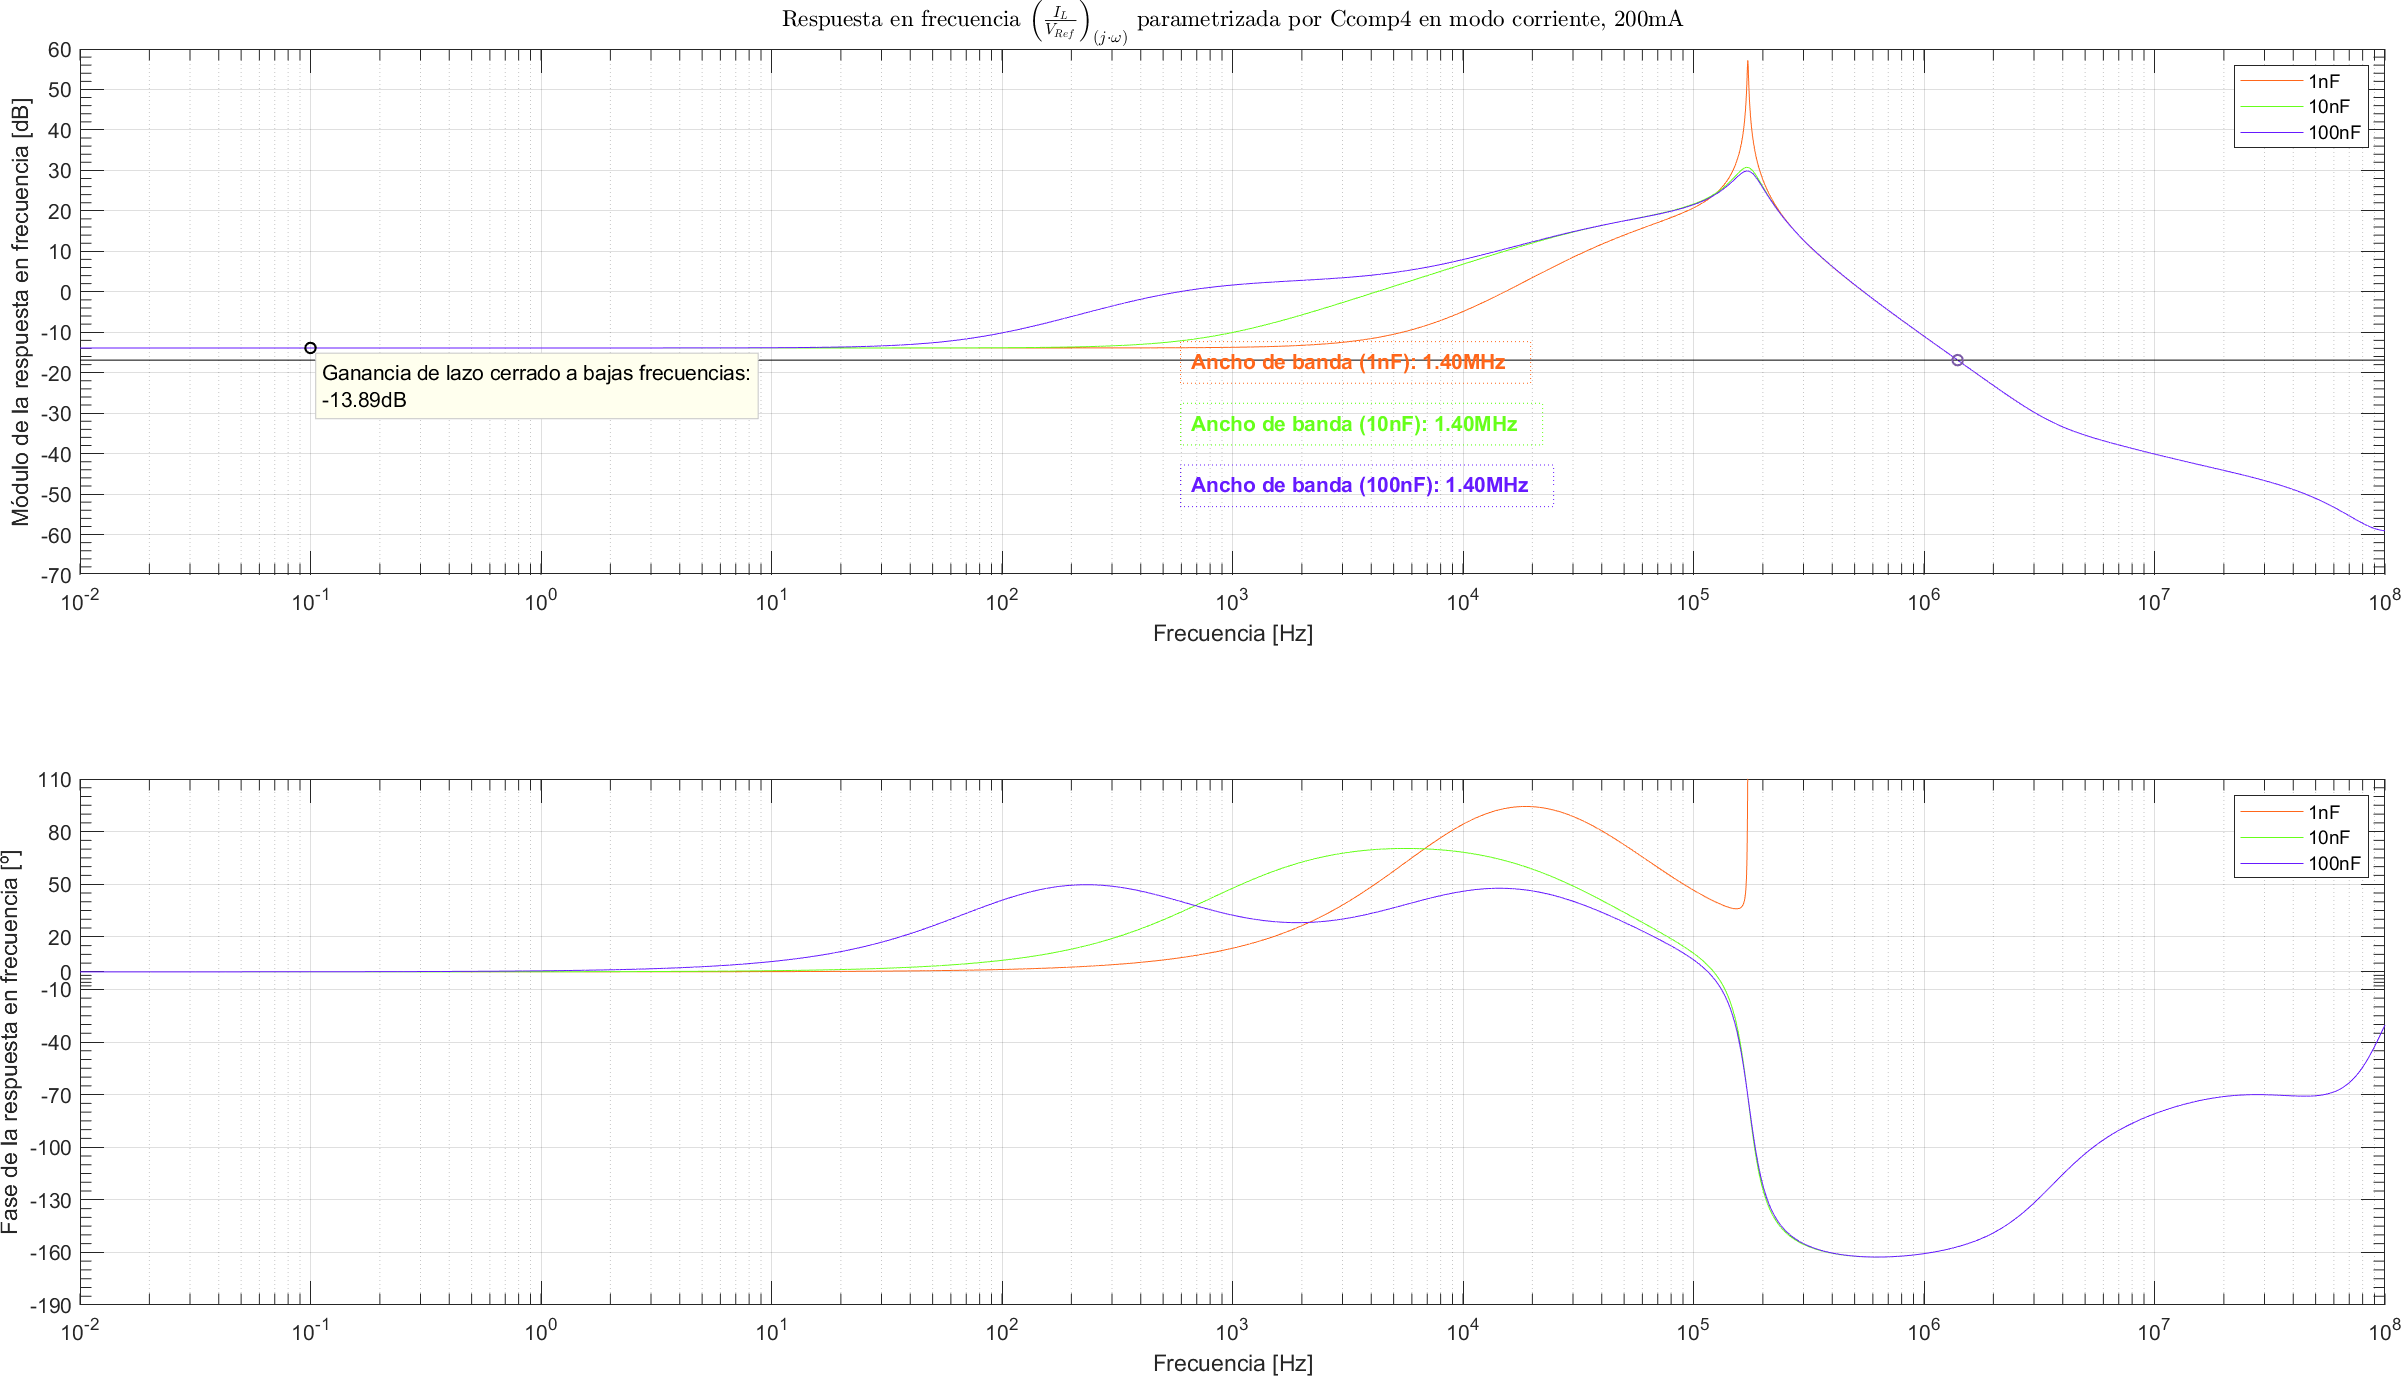
\includegraphics[width=1.1 \textwidth, angle=90]{./img/plots/rf/power_supply_CCOMP4_RF_Modo4.png}
\caption{\label{fig:fig_power_supply_CCOMP4_RF_Modo4}\footnotesize{Respuesta en frecuencia en modo corriente, $I_{out} = 200 \si[per-mode=symbol]{\milli\ampere}$, en función de la frecuencia parametrizada por $C_{comp_{4}}$.}}
\end{center}
\end{figure}

\clearpage

\begin{figure}[H] %htb
\begin{center}
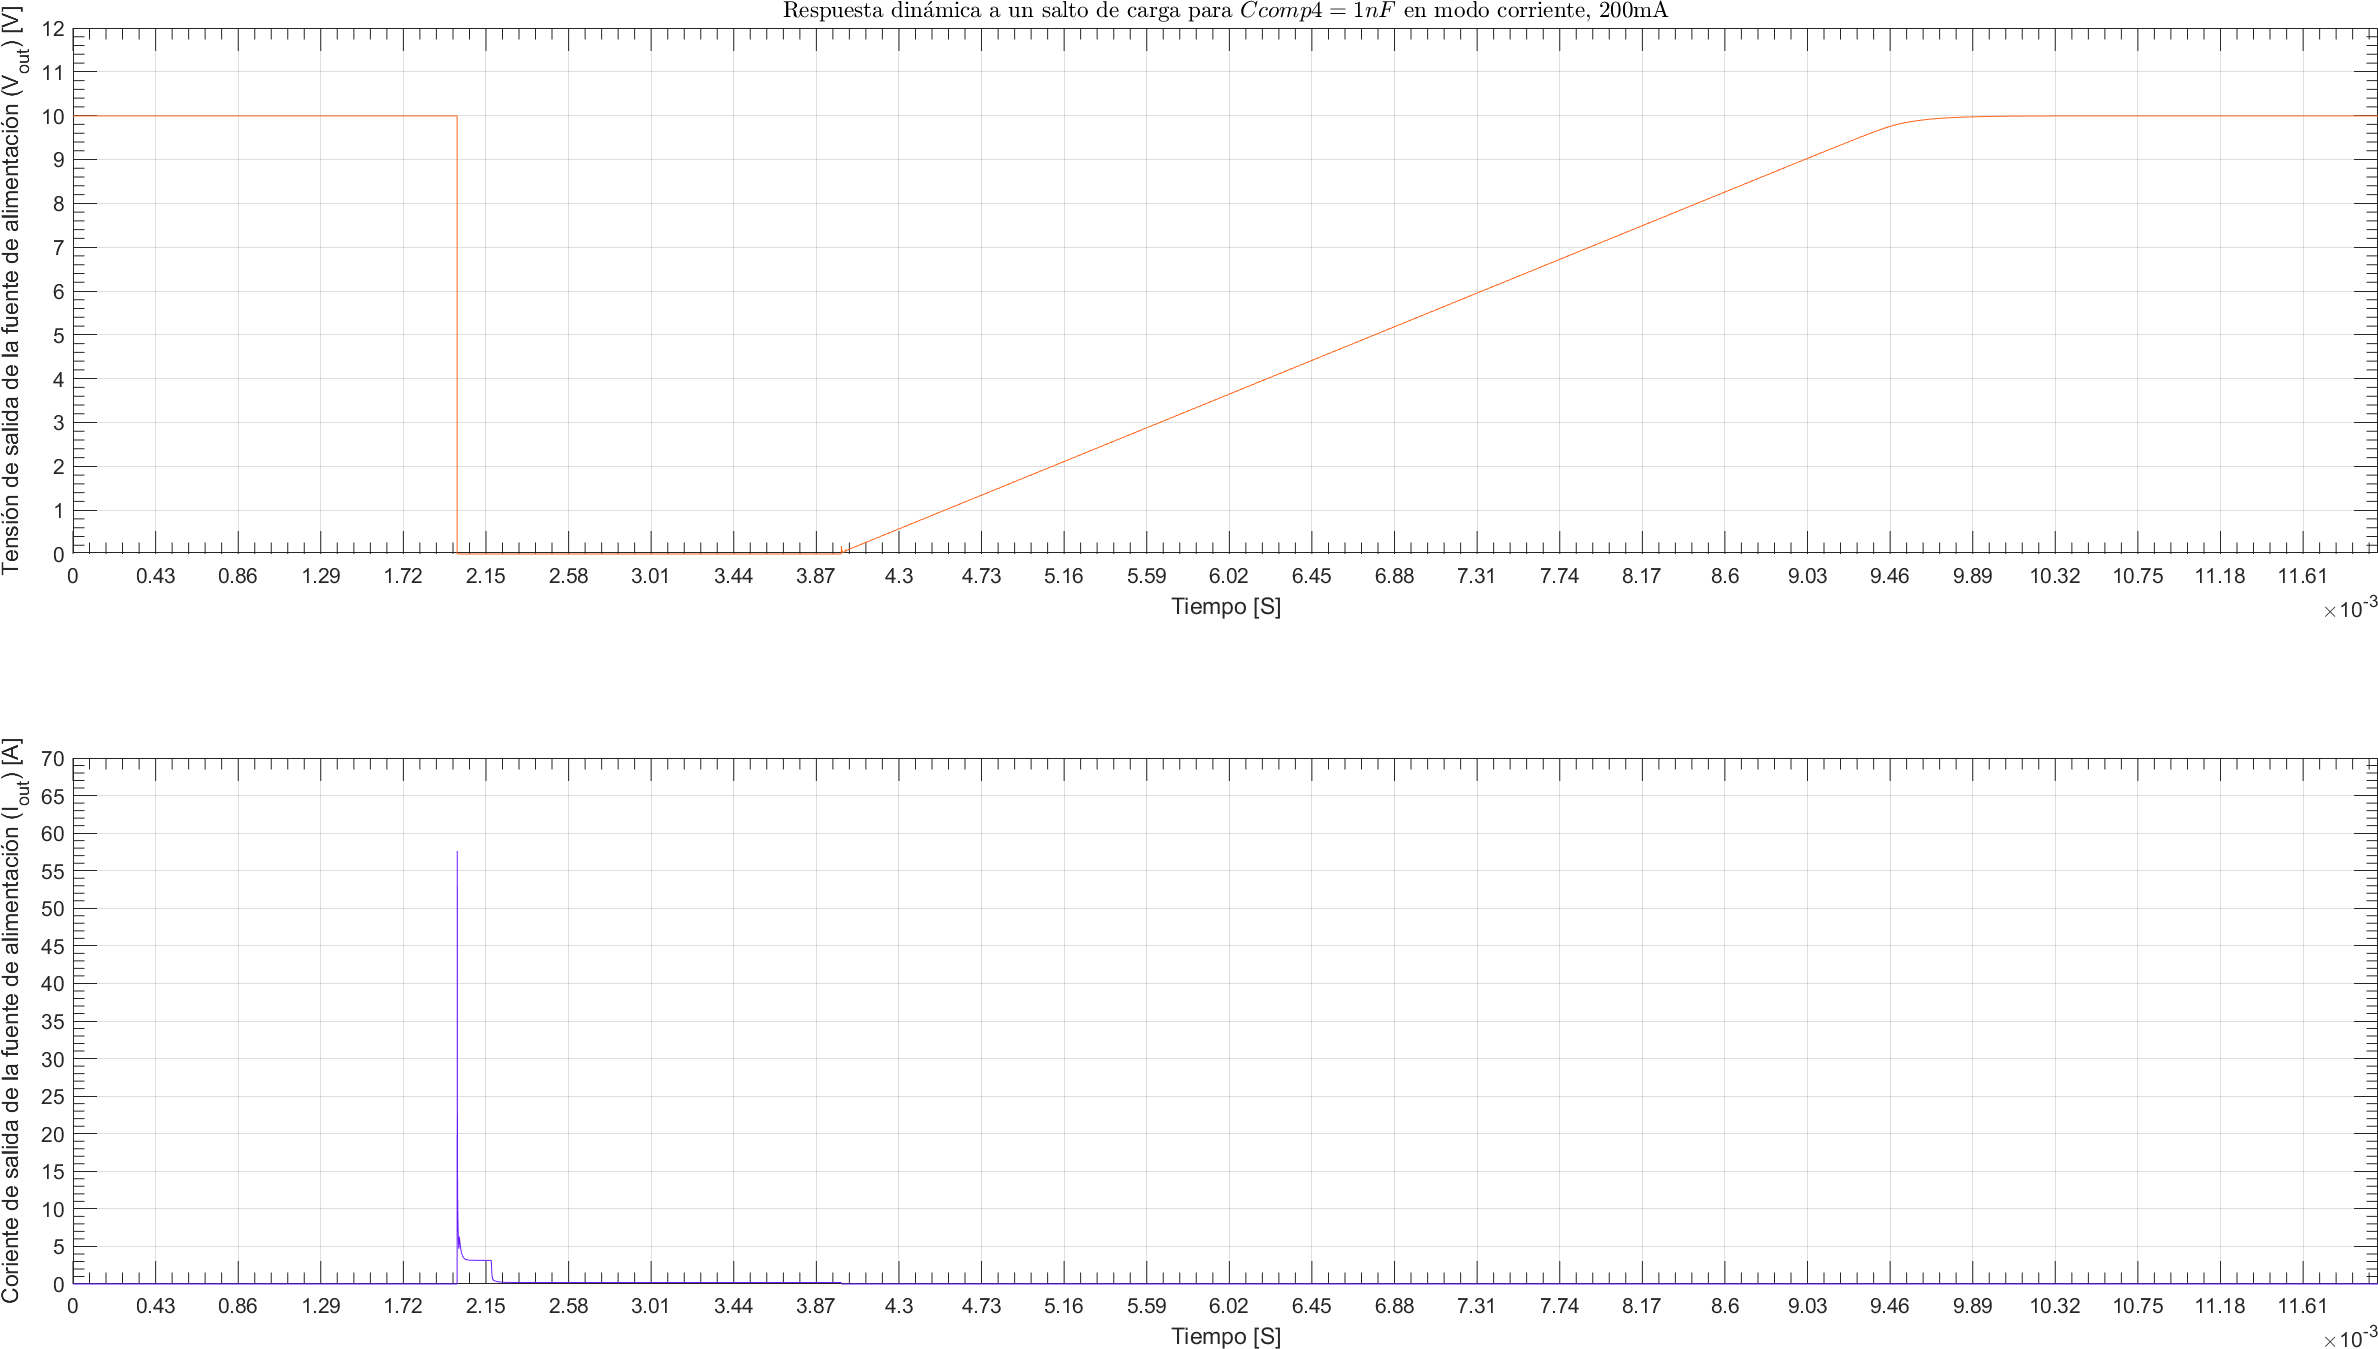
\includegraphics[width=1.1 \textwidth, angle=90]{./img/plots/dynamic/power_supply_CCOMP4_1n_STEP_Modo4.png}
\caption{\label{fig:fig_power_supply_CCOMP4_STEP_1n_Modo4}\footnotesize{Respuesta dinámica en modo corriente, $I_{out} = 200 \si[per-mode=symbol]{\milli\ampere}$, para $C_{comp_{4}} = 1 \si[per-mode=symbol]{\nano\farad} $.}}
\end{center}
\end{figure}

\clearpage

\begin{figure}[H] %htb
\begin{center}
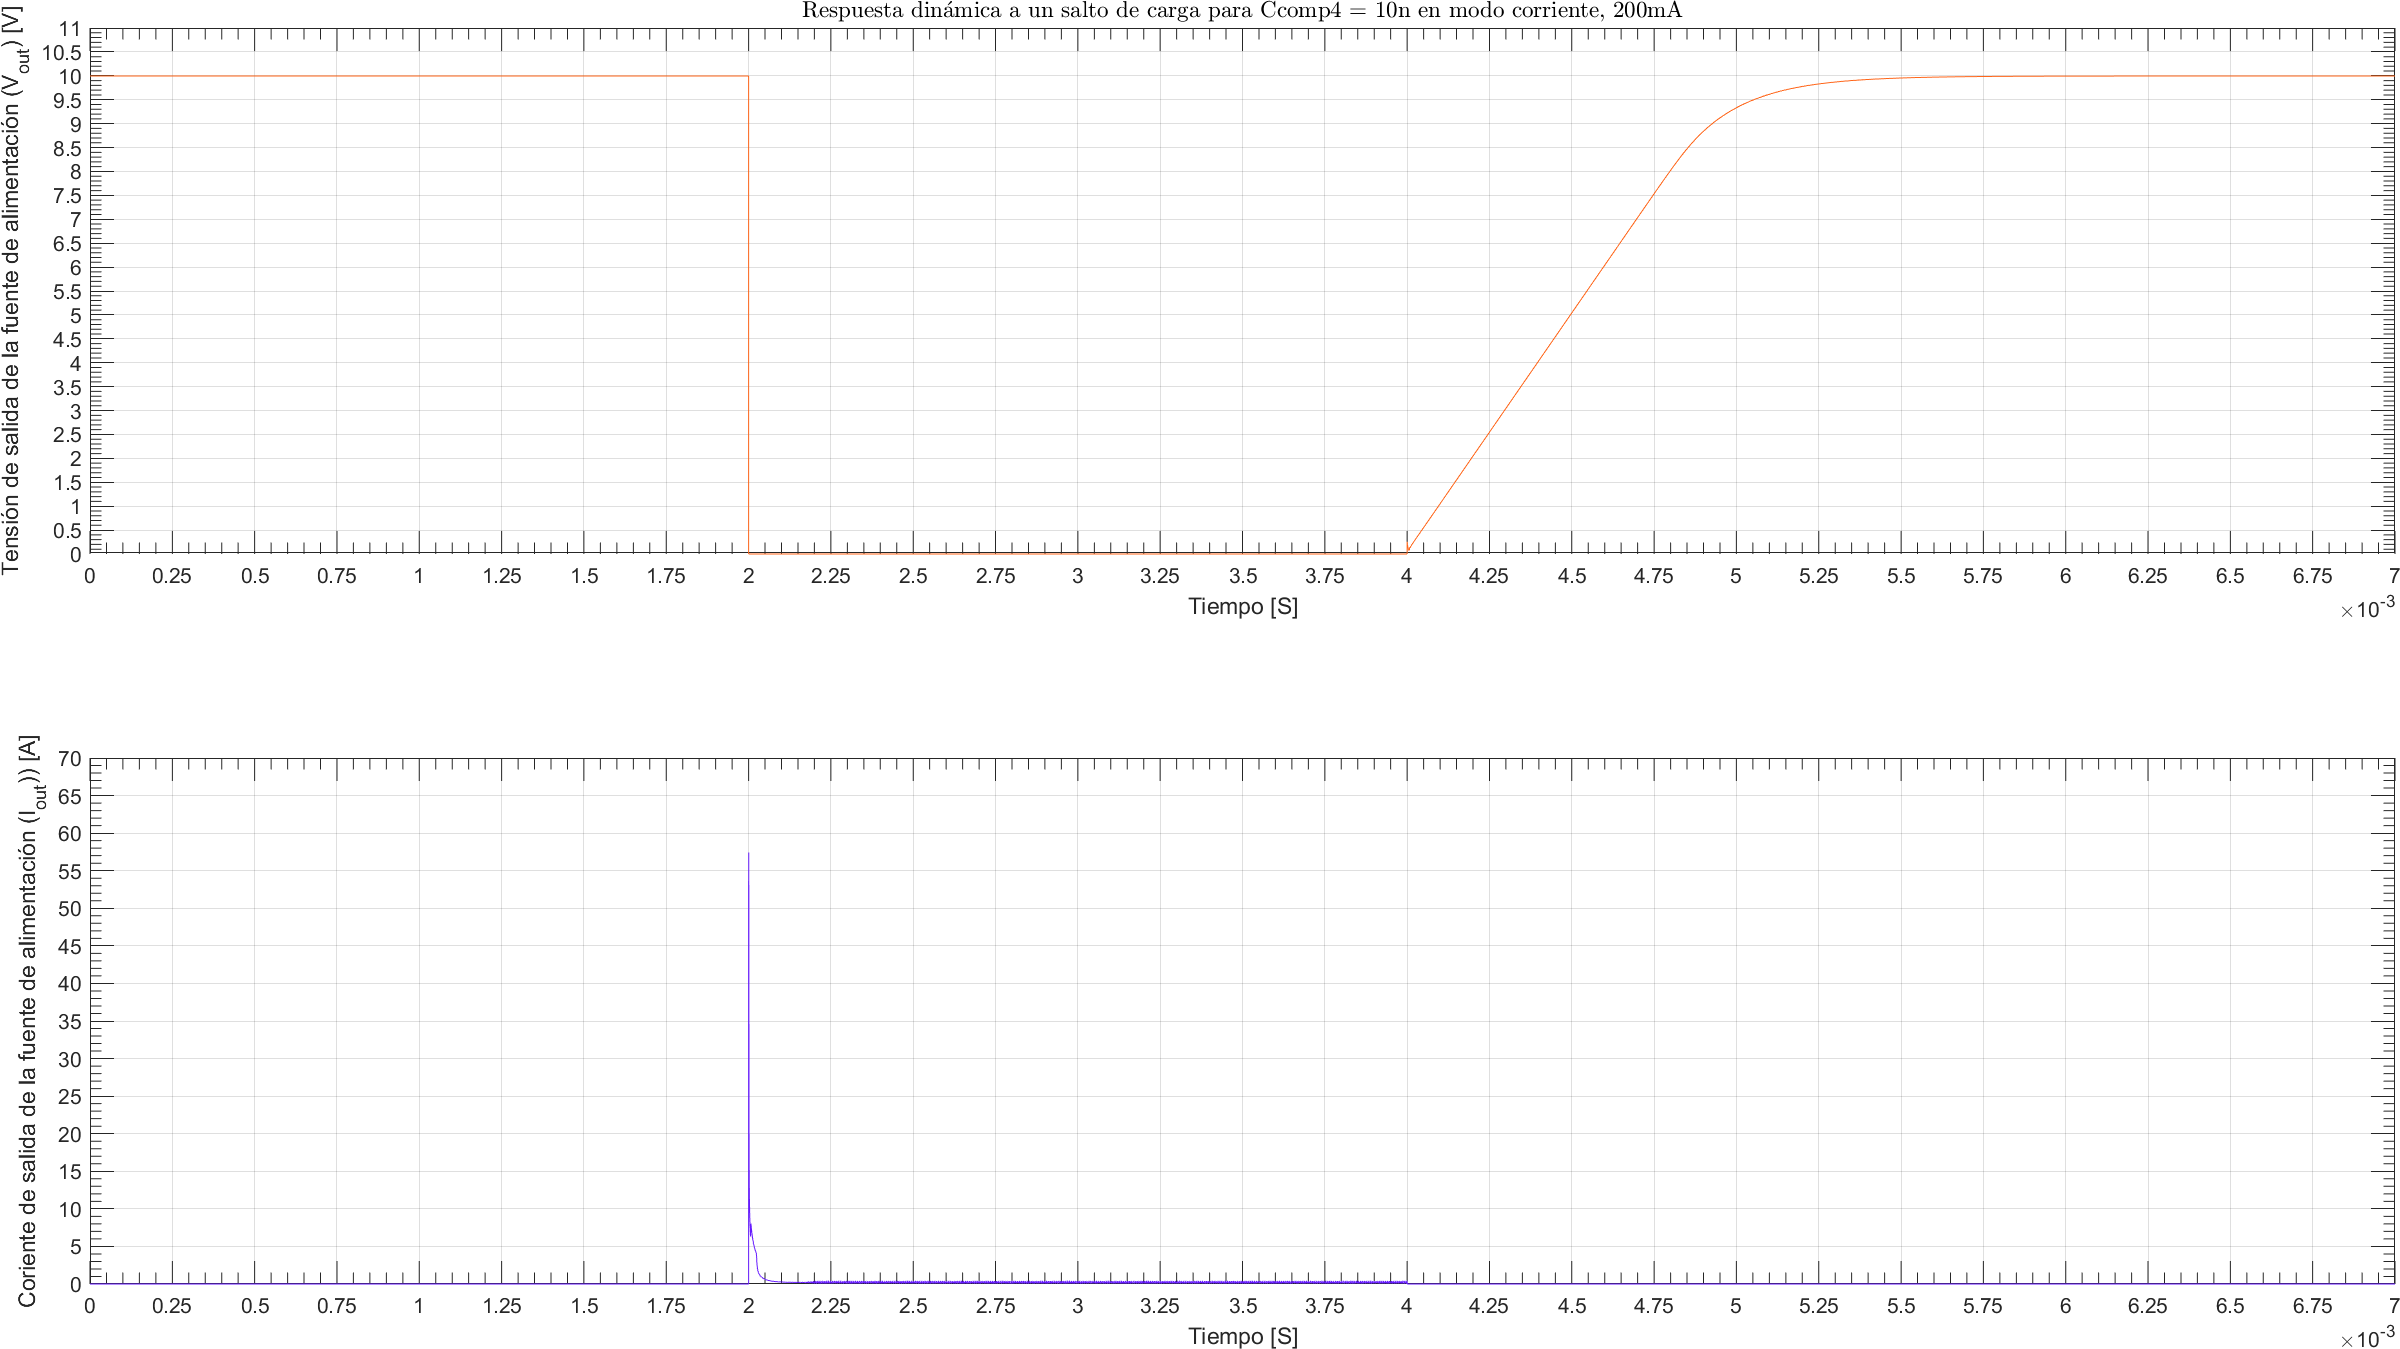
\includegraphics[width=1.1 \textwidth, angle=90]{./img/plots/dynamic/power_supply_CCOMP4_10n_STEP_Modo4.png}
\caption{\label{fig:fig_power_supply_CCOMP4_STEP_10n_Modo4}\footnotesize{Respuesta dinámica en modo corriente, $I_{out} = 200 \si[per-mode=symbol]{\milli\ampere}$, para $C_{comp_{4}} = 10 \si[per-mode=symbol]{\nano\farad} $.}}
\end{center}
\end{figure}

\clearpage

\begin{figure}[H] %htb
\begin{center}
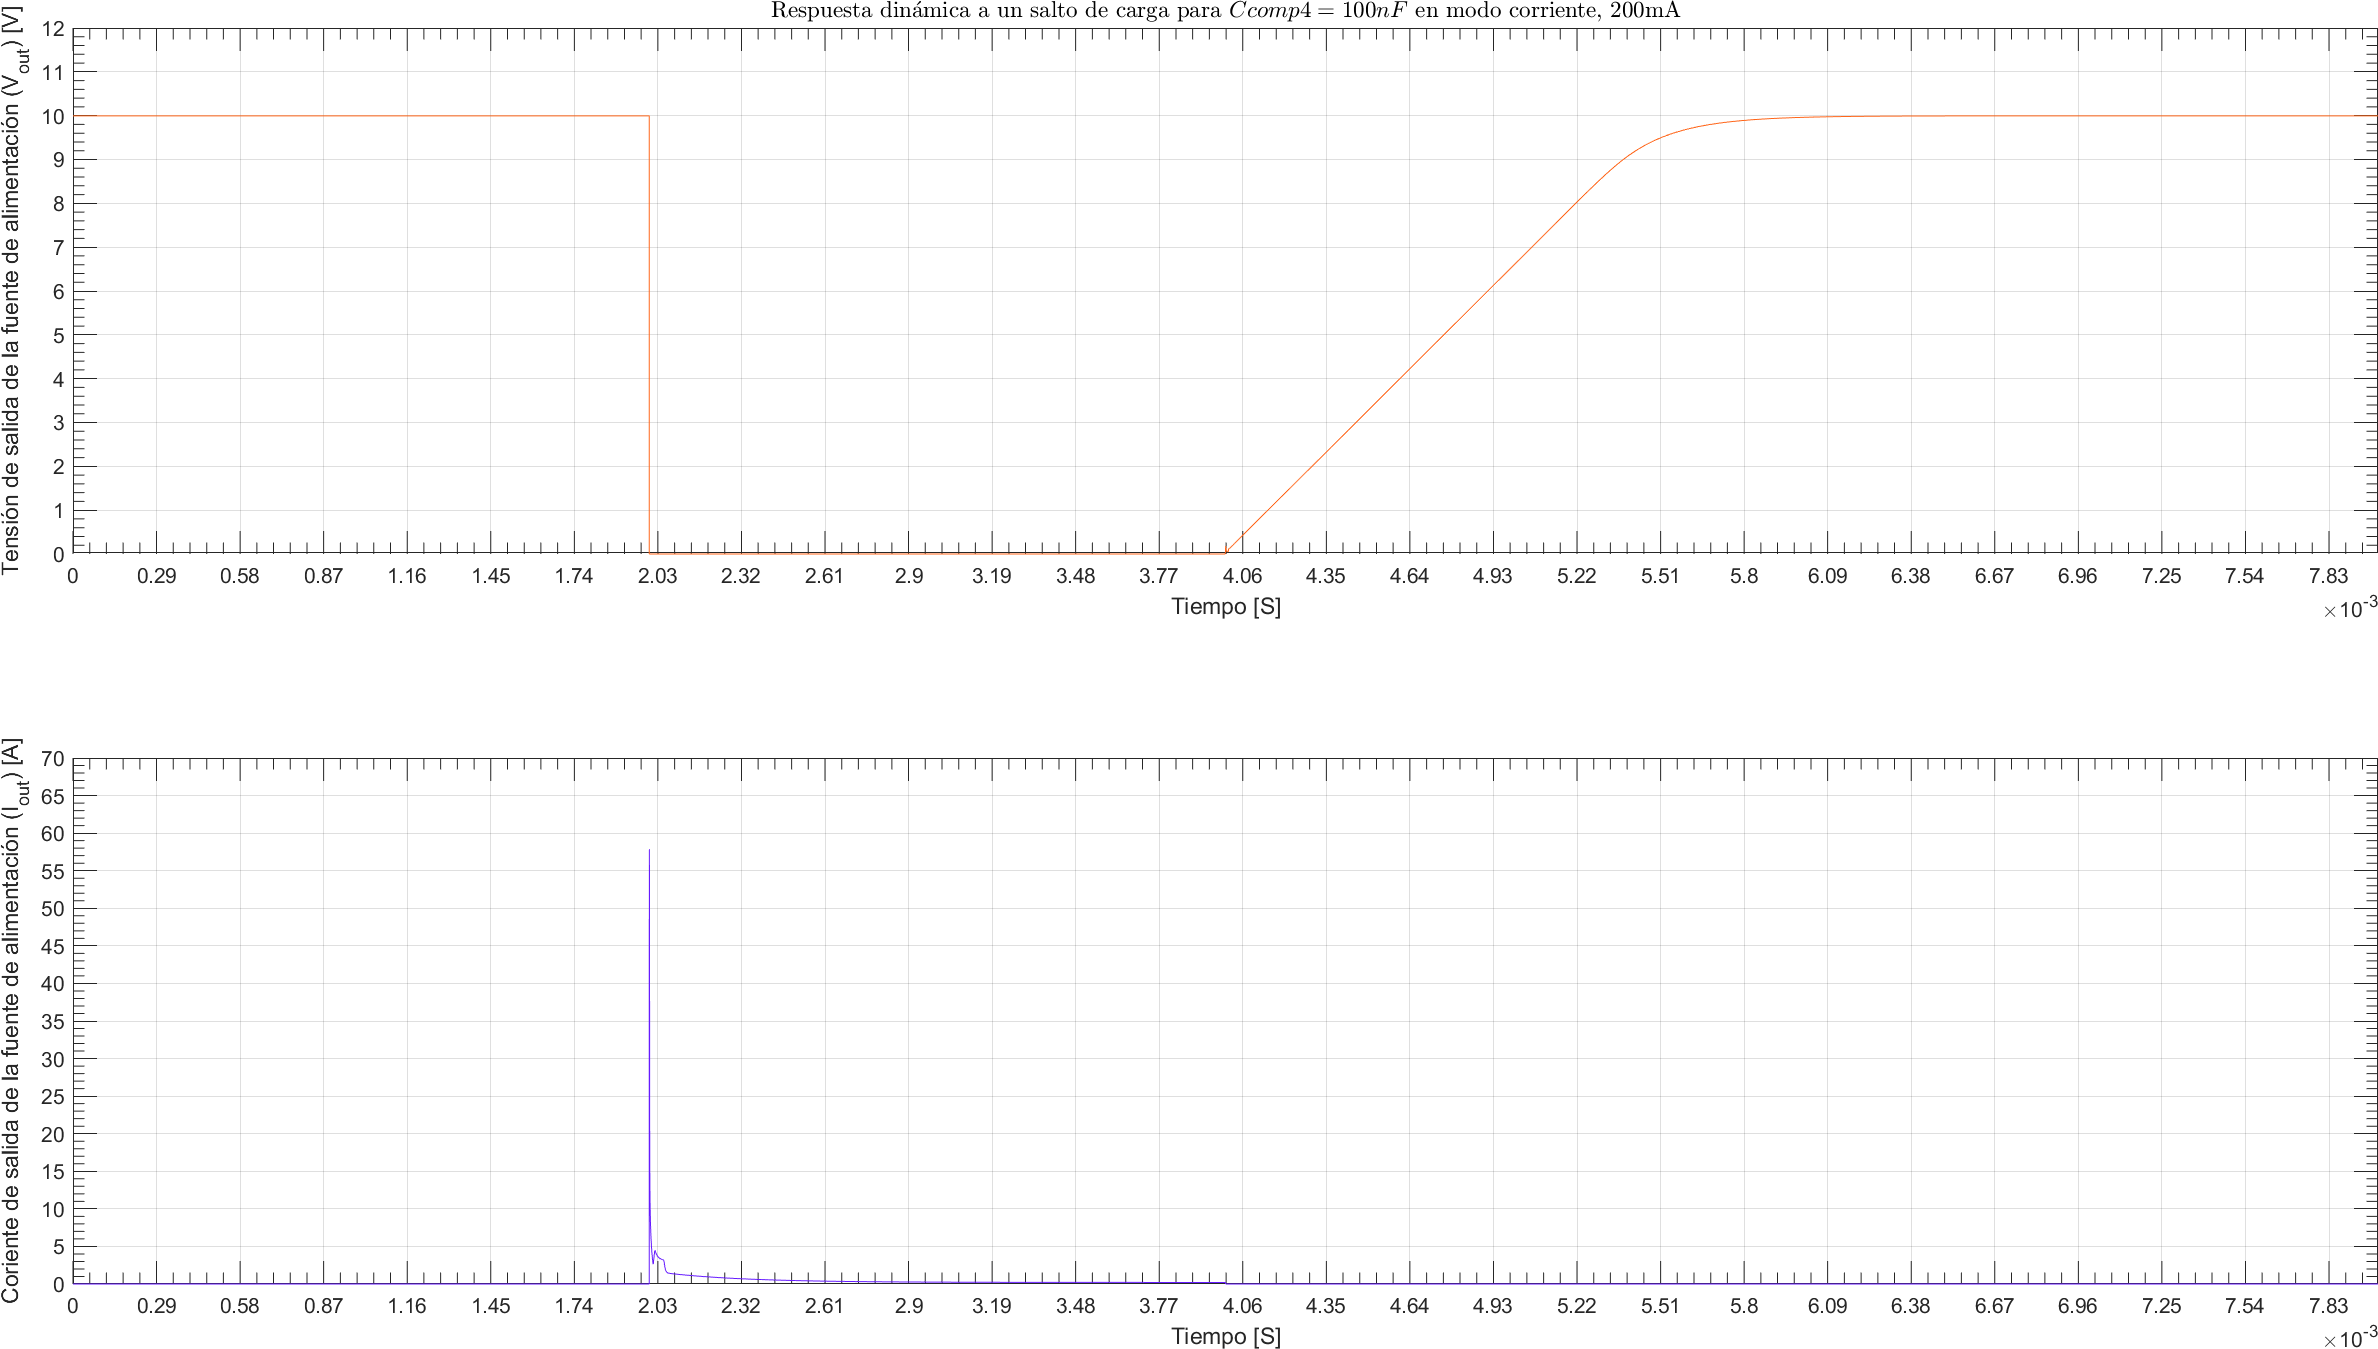
\includegraphics[width=1.1 \textwidth, angle=90]{./img/plots/dynamic/power_supply_CCOMP4_100n_STEP_Modo4.png}
\caption{\label{fig:fig_power_supply_CCOMP4_STEP_100n_Modo4}\footnotesize{Respuesta dinámica en modo corriente, $I_{out} = 200 \si[per-mode=symbol]{\milli\ampere}$, para $C_{comp_{4}} = 100 \si[per-mode=symbol]{\nano\farad} $.}}
\end{center}
\end{figure}

\clearpage




